
\begin{frame}{Introduction}

\vspace{-20pt}
\paragraph{Based on four key sources:}
\begin{itemize}
\item Mandelbrot 1967 (M67,~\cite{mandelbrot1967long}) -- Coasts, Fractals.
\item Emanuel 1986 (E86,~\cite{emanuel1986air}) -- Tropical Cyclones (TCs).
\item Taleb 2019 (T19,~\cite{taleb2019statistical}) -- Extreme Value Theory (EVT).
\item Yin et al.~2020 (Y20,~\cite{ZannaPreprint}) -- Inspiration.
\end{itemize}
\paragraph{Storm surges are created by (w.o.~tide-surge interaction):}
\begin{itemize}
\item  Wind stress creates $\sim 80$\% of a surge. In steady state\footnote{from Pugh, 1987~\cite{pugh1987tides} p.~89~\&~199.},

\begin{minipage}{0.45\linewidth}
\begin{equation}
\frac{\partial \eta}{\partial x}
\approx \frac{\tau}{\rho_{0} g H},
\notag
\label{eq:pugh}
\end{equation}
\end{minipage}
\begin{minipage}{0.45\linewidth}
\begin{equation}
\sim\implies \frac{\eta}{\tau} \approx \int \frac{d x}{H(x)\cdot g \cdot \rho_{\text {water}}}.
\notag
\end{equation}
\end{minipage}
\item Wave buildup $\sim 15$\% (not captured).
\item Pressure pull-up $\sim 5$\% (not recorded).
\end{itemize}
\paragraph{This report uses:}
\begin{itemize}
\item \texttt{surge}~\cite{gitlab}, \texttt{skextremes}~\cite{skextremes},
      \texttt{sklearn}~\cite{scikit-learn}, \& \texttt{xarray}~\cite{hoyer2017xarray}.
\item \texttt{two-year} `04-`05 (\texttt{tyr}), \&  \texttt{control-1950} 101-yrs (\texttt{c50}).
\end{itemize}

\end{frame}



\begin{frame}{}

\begin{minipage}{0.45\linewidth}

\includegraphics[width=\linewidth]{../surge/plots/angle_heatmap.pdf}\\
$\uparrow$~Bearing \& $\downarrow$~Convexity \texttt{eUS}.

\includegraphics[width=\linewidth]{../surge/plots/derivative_heatmap.pdf}

\end{minipage} \begin{minipage}{0.45\linewidth}
\raggedleft
\includegraphics[width=\linewidth]{../surge/plots/bath_list.pdf}\\
{$\uparrow$ Isobaths on \texttt{eUS}.}

{$\downarrow$ Distance from \texttt{eUS}.}
\includegraphics[width=\linewidth]{../surge/plots/distance_isobath.pdf}\\

\end{minipage}

\end{frame}

\begin{frame}
%\hspace{-40pt}
\begin{minipage}{0.6\linewidth}
\includegraphics[width=\linewidth]{../surge/plots/rmlr.pdf}
 %\vspace{-15pt}

\label{fig:tau-tau-resp}
\end{minipage}
%\hspace{-40pt}
\begin{minipage}{0.3\linewidth}
\raggedright
{$\leftarrow$ Regressing
  \Large{~~~X:~$\boldsymbol{\tau}$,~~~~Y:~$\eta_{\;\mathrm{hp}}$}}
\hspace{50pt}

\raggedleft
\includegraphics[width=\linewidth]{../surge/plots/reg_angle.png}\\
{$\uparrow$ Normal bearing and regression line similar.}
\end{minipage}

 \label{fig:tau-tau-angle}
 \begin{minipage}{0.6\linewidth}
 \includegraphics[width=\linewidth]{../surge/plots/adj_reg_mag.pdf}
 \end{minipage}
 \begin{minipage}{0.3\linewidth}
 {$\leftarrow$ Responsiveness magnitude.}
 \end{minipage}
\end{frame}

\begin{frame}
\centering \vspace{-20pt}
\begin{align}
    \operatorname{GEV}(x; \mu, \sigma, \xi)&=&
    \frac{1}{\sigma} \chi(x)^{1-\xi} e^{-\chi(x)}; \tag{GEV-1} \label{eq:GEV-1} \\
    \chi(x)&=&\left\{\begin{array}{ll}
    \left(1-\xi\left(\frac{x-\mu}{\sigma}\right)\right)^{1 / \xi} & \text { if } \xi \neq 0 \\
    e^{-(x-\mu) / \sigma} & \text { if } \xi=0 \tag{GEV-2}
    \end{array}\right.
   \label{eq:GEV-2}
\end{align}

\includegraphics[width=0.8\linewidth]{../surge/plots/GEV_modelNO.pdf}\\
NO GEV plot \texttt{skextremes}~\cite{skextremes}
        for \texttt{c50}.
         A~\&~C show bad fit?

\end{frame}

\begin{frame}{\texttt{c50}, \texttt{eUS}, GEV parameters}
\vspace{-20pt}

\includegraphics[width=0.8\linewidth]{../surge/plots/skextreme_second_tactic.pdf}\\
CI of GEV show that fit is poor.
$\xi$ is more negative
in Gulf of Mexico. $r_p$
show that $\mu$ and $\sigma$ are correlated (all $r_p$ have 1\%$\gg$p).
$\mu$ and responsiveness: $r_p=0.44\pm0.02$, p$<10^{-30}$.
\end{frame}

\begin{frame}{The Potential Intensity of Tropical Cyclones (TCs)}
\vspace{-30pt}
\hspace{-30pt}\begin{minipage}{1.1\linewidth}
\centering
\begin{minipage}{0.45\linewidth}
\centering
    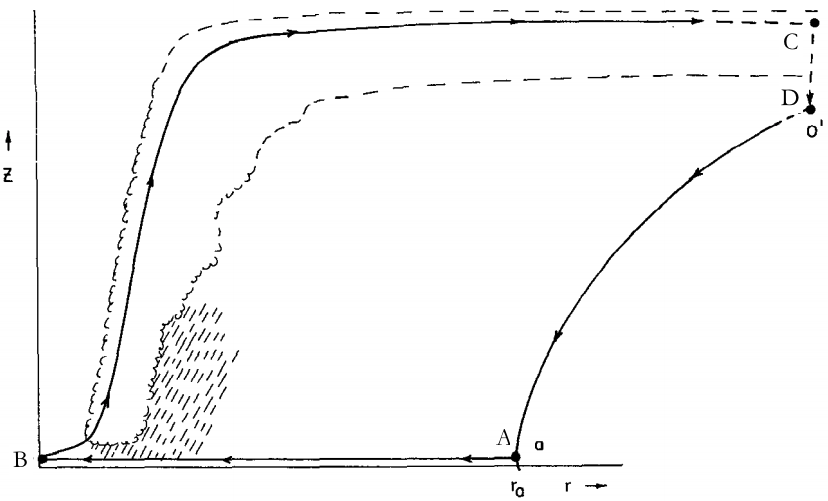
\includegraphics[width=\linewidth]{images/hurricane-carnot.png}\\
    \textit{Figure 1 from~\cite{emanuel1991theory}.
    TCs are a Carnot cycle. }
    \end{minipage}
\begin{minipage}{0.45\linewidth}
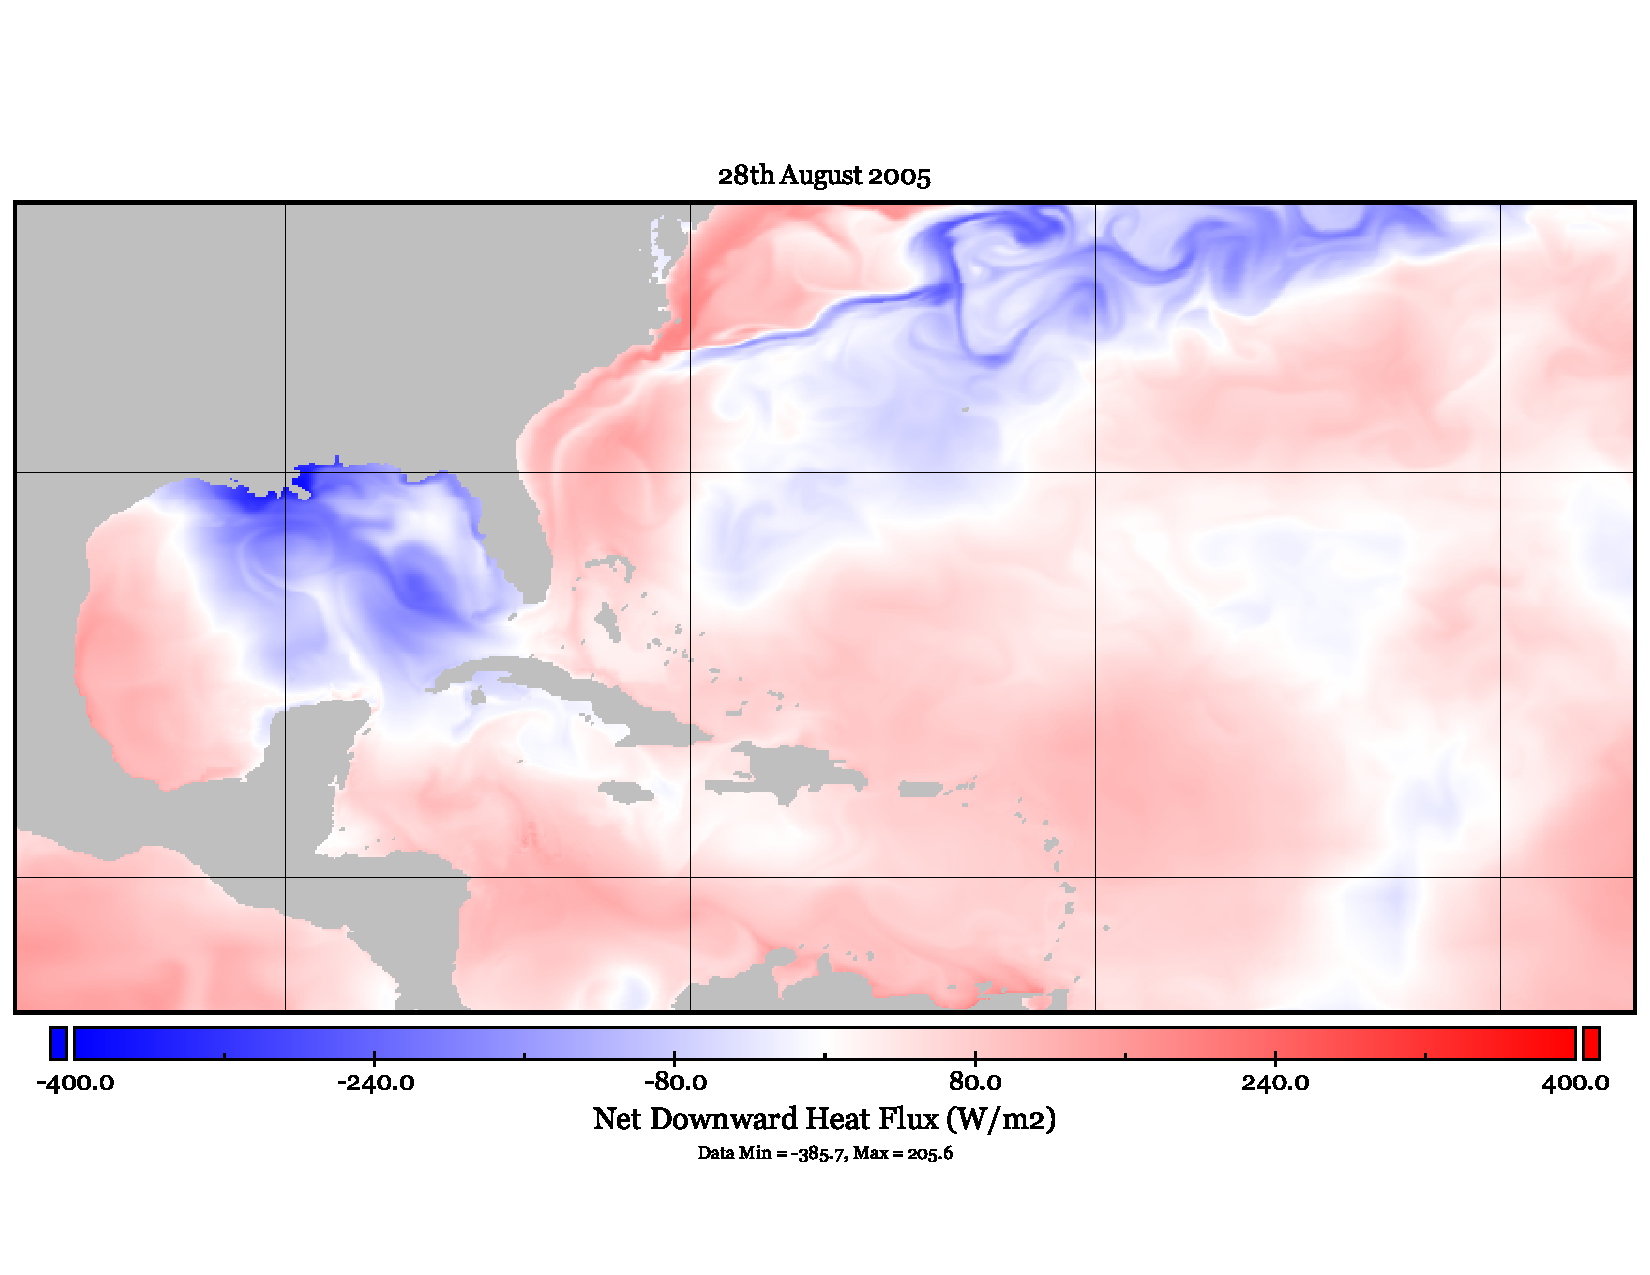
\includegraphics[width=\linewidth]{kat-heat.pdf}\\
\textit{Daily downwards heat flux
        \texttt{tyr}.}
       \end{minipage}
\end{minipage}
\begin{itemize}
\item TCs are a finite amplitude wind induced heat exchange (WISHE) instability.
\item The potential intensity (equation 15-7 in \cite{emanuel2018progress}) is,

\begin{minipage}{0.45\linewidth}
\begin{equation}
\left|\mathbf{V}_{s}\right|^{2}=\frac{C_{k}}{C_{D}}
\frac{T_{s}-T_{o}}{T_{o}}\left(k_{0}^{*}-k_b\right),
\tag{PI}
\label{eq:PI}
\end{equation}
\end{minipage}
\begin{minipage}{0.45\linewidth}
\begin{equation}
k \equiv c_{p} T+L_{v} q,
\label{eq:enthalpy_per_unit_mass}
\end{equation}
\end{minipage}
\end{itemize}
\end{frame}

\begin{frame}{%Yearly PI $\implies$ BM plateau.
}
\centering
\vspace{-1pt}
 \begin{minipage}{0.45\textwidth}
    \centering
    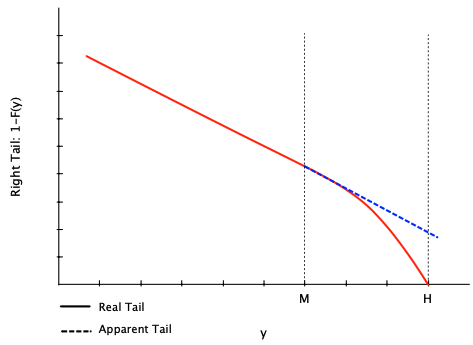
\includegraphics[width=1\linewidth]{images/taleb-limit-slimmed.png}\\
    \textit{Figure 15.1 from T19~\cite{taleb2019statistical} p.~279}
   \end{minipage} \begin{minipage}{0.45\textwidth}
   \includegraphics[width=1\linewidth]{../surge/plots/GEV_pi_plateau_NO.pdf}
   Attempt at enforcing a GP asymptote of 1.9m for NO.
   %1$\sigma$ and 2$\sigma$ envelopes shown.
   %\label{fig:gp-plateau}
   \end{minipage}
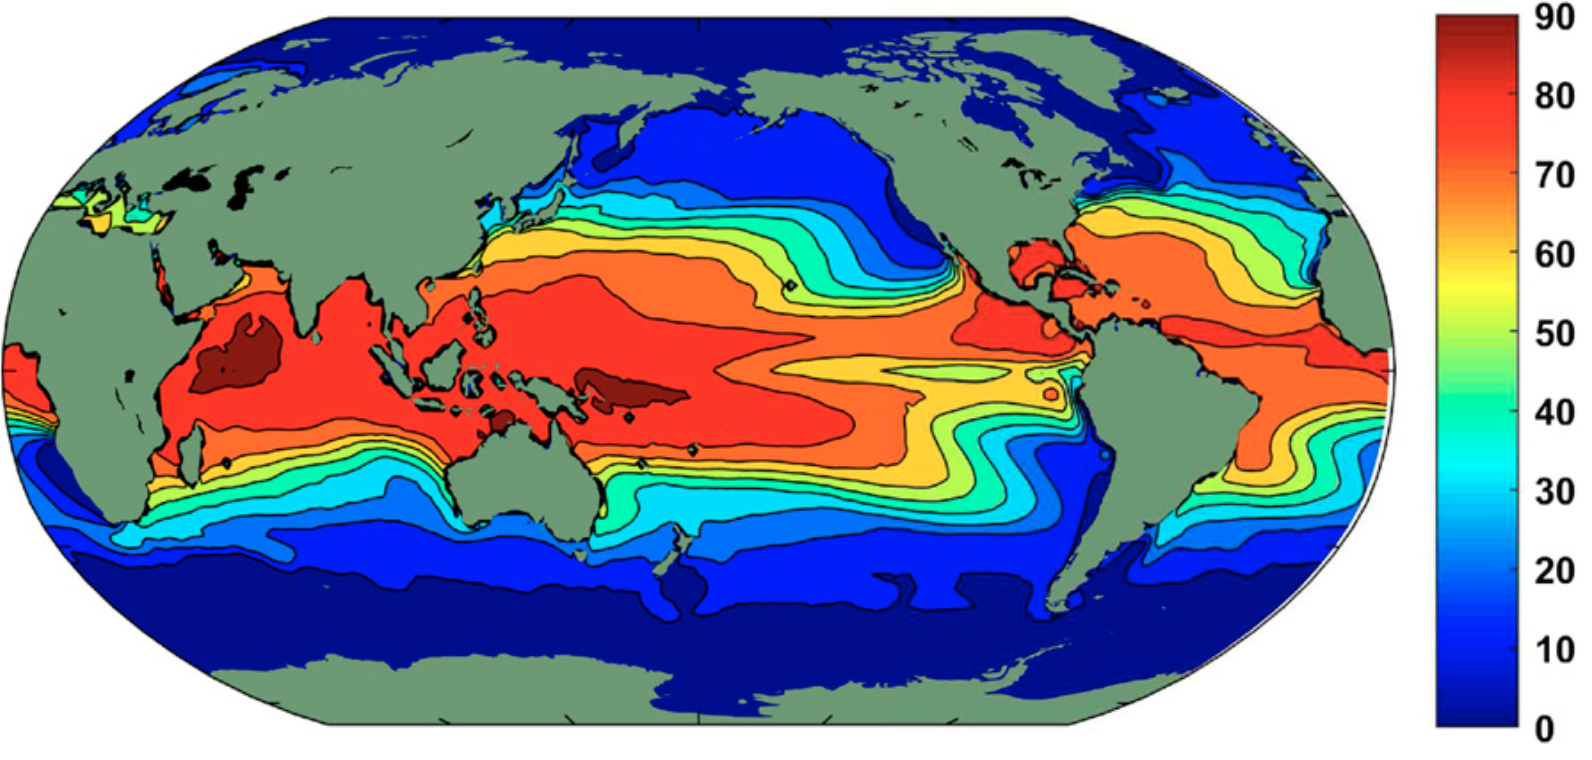
\includegraphics[width=0.7\linewidth]{images/PI-max-year.png}\\
\textit{Figure 15-7 from \cite{emanuel2018progress}.}
Annual maximum of the PI (m s$^{-1}$), calculated using~\cite{bister2002low}
and ERA-Interim data 1979-2016~\cite{dee2011era, berrisford2009era}.

\end{frame}


\begin{frame}{Summary}
\centering
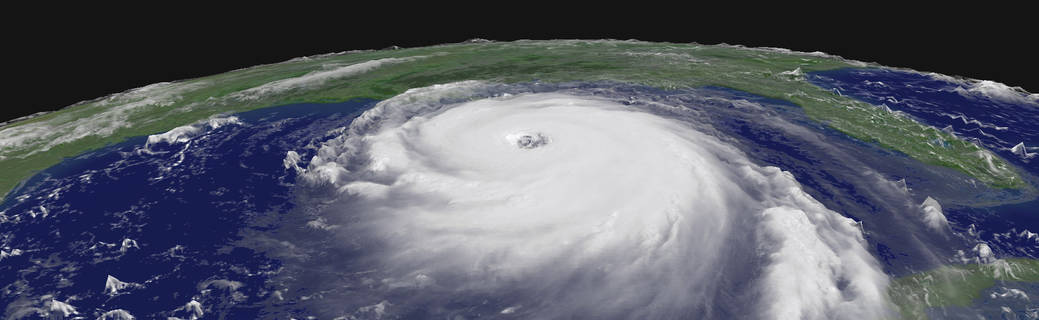
\includegraphics[height=2cm]{images/NASA-KATRINA-SIDEON.jpg}
\begin{itemize}
\item Extract the coastline, and characterise it quantitatively.
\item Responsiveness behaves simply.
\item Block maxima to estimate hazard.
\item Hazard made tractable through physical constraints.
\end{itemize}
\centering
\includegraphics[height=3cm]{../surge/plots/theory.pdf}

\end{frame}
